% !TeX root = ../thuthesis-example.tex

\chapter{相关研究综述}
本节首先介绍了目前各类型主流数据管理系统的数据写入形式与接口设计,然后介绍了若干为了提高数据写入吞吐而设计的高性能存储引擎,最后介绍了与数据库客户端以及 RPC 相关的优化。
\section{数据写入机制概述}
本节首先介绍关系型数据库中主流 OLTP 数据库和 OLAP 数据库的数据写入设计,然后介绍主流时序数据库和数据湖的数据写入设计。
\subsection{关系型数据库写入概述}
主流的关系型数据库根据设计目标的不同,可以分为 OLTP(On-Line Transaction Processing)数据库和 OLAP(On-Line Analytical Processing)数据库\cite{silberschatz2011database}。如图\ref{fig:data-pipelines-oltp-olap}所示,在一般的应用架构中,用户的应用在线运行时,一般直接与 OLTP 数据库进行交互,完成数据的写入、修改、删除、查询等工作。因此,OLTP 数据库的数据写入通常是以事务的形式进行的。除 OLTP 数据库外,为了满足分析报表、企业 BI 等应用需求,用户还会运行一个 OLAP 数据库,并且将 OLTP 数据库中的数据定期地通过 ETL(Extract-Transform-Load)工具导入到 OLAP 数据库中。因此,OLAP 数据库的数据写入通常是以批量的形式进行的。
\begin{figure}
  \centering
  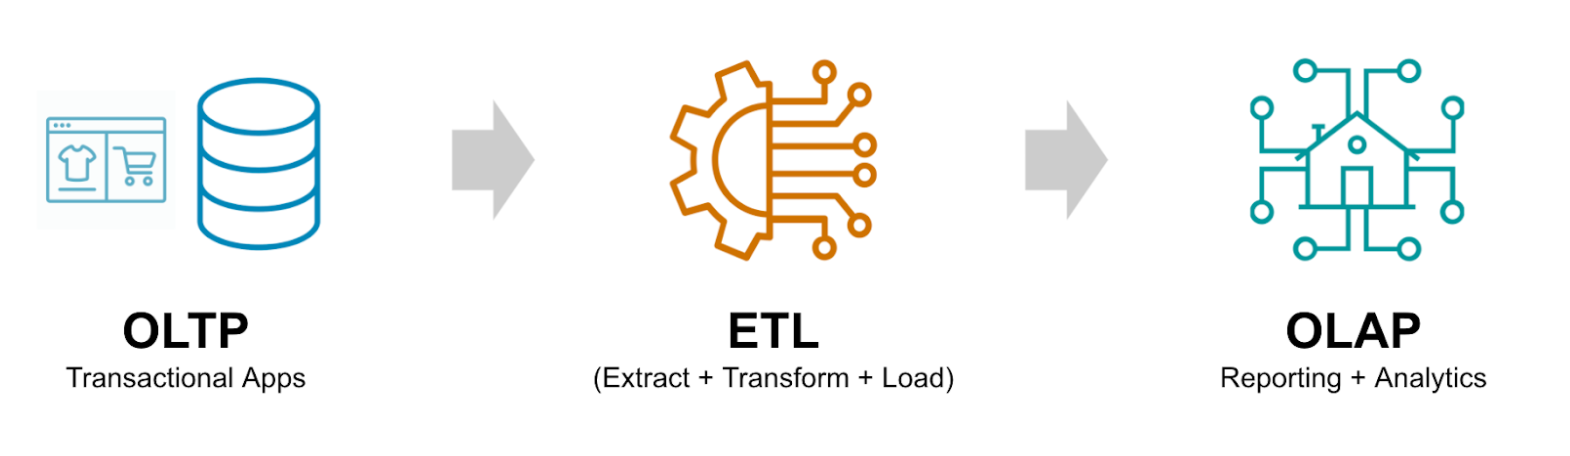
\includegraphics[width=\textwidth]{data-pipelines-oltp-olap.png}
  \caption{常见的数据处理流程}
  \label{fig:data-pipelines-oltp-olap}
\end{figure}

\subsubsection{OLTP 数据库写入}
如上文所述,对 OLTP 数据库的写入主要通过事务进行,因此事务的形式就决定了写入的形式。事务这一概念最早出现于二十世纪七十年代,其最初是为了支持集中式系统中简单的“借贷”式数据库操作而开发的,这些数据库通常为金融领域的应用而服务\cite{wang2008survey}。到如今,事务机制已经成为了 OLTP 数据库系统不可或缺的重要组件,其所能支持的应用范围也不再仅限于金融领域。

随着事务的发展,研究者也提出了各种各样的事务模型。扁平事务(Flat Transaction)模型是最基础和最常见的事务模型,它支持事务的 ACID(Atomicity,Consistency,Isolation,Durability)特性\cite{gray1981transaction},每个事务之间都是独立的,没有关联性\cite{wang2005historic}。虽然扁平事务非常简单,但是它无法满足一些应用对长期运行事务(Long-living transaction)或复杂事务的需求,因此研究者提出了其他更加复杂的事务模型。
这些复杂事务模型的基本思想是将一个事务划分为多个子事务,子事务在有需要的时候进一步划分为更小的事务,这样的模型可以更好地支持复杂的或者长期运行的事务\cite{klas1992database}。例如,如果一个长期运行的事务在操作中出现了错误,那么它可以仅重新执行其中的一个子事务,而不是将整个事务都重新执行。这一类复杂事务模型的代表有:
\begin{enumerate}
  \item 分布式事务模型(Distributed Transaction Model)。这一类事务模型在一个全局事务中包含了多个局部子事务,每个子事务都是在一个独立数据库节点上运行的。当所有子事务成功提交时,全局事务才能成功提交\cite{breitbart2010overview}。
  \item 嵌套事务模型(Nested Transaction Model)。\cite{weikum1992concepts}
\end{enumerate}
\subsection{时序数据库写入}
\section{高性能存储引擎设计(围绕时序数据库)}
\subsection{基于 B+ 树的存储引擎设计}
\subsection{基于 LSM 树的存储引擎设计}
\section{数据库客户端与 RPC 优化}